% !TEX root = ../main.tex
\chapter{Background}
Before we start, there are some basics that are useful to know about.
In this chapter we introduce the formalism for our model and for our properties to verify.
We also explain the ideas behind mutexes, deadlocks and compilers.
And we begin our background chapter with a summary of the programming language Rust.

\section{Rust}
\label{rel_rust}
By trend, programming languages can be divided into fast or safe\cite{speedSafety}: 
either a language is used to produce highly optimized code that runs fast on the targeted system,
or a language makes use of sophisticated safety features that prevent inconsistencies at the cost of runtime performance.

The Rust project is an attempt to build a language that is both: fast and safe, 
as the official slogan indicates: ``A language empowering everyone
to build reliable and efficient software'' \cite{rustSite}.
To ensure a minimal performance overhead Rusts runtime was kept small\cite[Chapter 16.1]{klabnik2018rust} and features like garbage collection where neglected\cite[Chapter 4]{klabnik2018rust}.
Instead, safety issues are addressed with Rusts \textbf{ownership model}\cite{Matsakis:2014:RL:2692956.2663188}.

In Rust, a memory resource (object) is associated by one unique owning variable.
The owner can mutate the object, reference it or hand over ownership.
When handing over ownership it is lost for the previous owner (to unsure unique ownership).
However, references can be `borrowed' without loosing ownership.
These borrows come in two flavors:
\begin{enumerate}
  \item There can be an arbitrary amount of \textbf{immutable references} at a given time.
  \item But only one active \textbf{mutable reference}. 
  No immutable references can be active at the same time and the owner is prohibited from mutating while a mutable borrow is active.
\end{enumerate}
References that go out of scope are ensured to be deconstructed by Rusts \textbf{borrow checker}. 
Programs that do not meet the ownership requirements will not compile and raise an appropriate error message.

By enforcing the ownership rules, Rust programs avoid common problems like dangling pointers, double frees and data races\cite{Matsakis:2014:RL:2692956.2663188} with no impact on execution speed.
The cost is transferred to compile time, where additional errors complicate development and established programming patterns have to be revised.
And while eliminating all these errors can be invaluable, Rust cannot prevent all mistakes.
One of which are deadlocks\cite[Chapter 8.1]{nomicon} which we want to address with this work.

\section{Deadlock and Mutex}
Typically, deadlocks are a problem of concurrent systems where resources are shared or a section of a program must only be entered once at a time (a critical section).
To assure sequential access, those resources are often guarded by a locking mechanisms like Dijkstras semaphores\cite{dijkstra1968cooperating} or the simpler form: a mutex (for mutual exclusion). Mutexes are used for exclusive access to a critical section.
If a process wants to enter this section, it has to acquire a mutex lock.
This is only possible if no other process currently has acquired the lock, otherwise the former process has to wait (or try later).
After the process left the critical section, the lock has to be released to unblock waiting processes.
If the locks are not released correctly it can lead to a situation where all process are waiting to acquire a mutex lock that will never be released and the whole execution comes to a halt: a deadlock.
A deadlock situation often depends on nondeterministic behavior (for example process/thread scheduling or network communication) which can make debugging rather difficult.
Therefore, having proof of deadlock absence can be powerful information, especially in highly parallel systems.

\section{Compilers}
The goal of this work is to combine the benefits of Rusts ownership system with the benefits of Petri-Net model checking.
To achieve this goal we have to translate from Rust to Petri-Nets, 
and we want to do it programmatically.
This is basically the definition of a compiler\cite[Chapter 1.1]{aho1986compilers}:
\begin{quote}
``Simply stated, a compiler is a program that can read a program in one language -- the source language -- and translate it into an equivalent program in another language -- the target language;''
\end{quote}
Compilers underwent heavy research and development in the past.
Nowadays the structure of a compiler can be summarized into well-defined phases\cite[Chapter 1.2]{aho1986compilers}:

\begin{enumerate}
  % TODO: überall beispiele?
  \item During the \textbf{Lexical Analysis}, the character stream of a source file is converted into a token stream.
  Tokens are all significant language components like keywords, identifiers and symbols (`=', `+', `\{', etc.).
  \item During \textbf{Syntax Analysis} (parsing) the token stream is structured into a tree,
  typically a syntax tree, where each node represents an operation with its children as operation arguments.
  \item The following \textbf{Semantic Analysis} checks that the syntax actually matches the requirements (the grammar that the language is based on).\newline
  Additional static analysis -- like type checking -- is done in this phase as well.
  \item Further representations might be produced in the \textbf{Intermediate Code Generation} phase.
  An intermediate representation can be everything that helps.
  A low level representation that is close to machine code is a common case.
  Examples are Java Bytecode or the LLVM intermediate representation
  \item The intermediate representation can be used for further analysis and optimization in the \textbf{Code Optimization} phase.
  Executable size or execution speed might be improved here.
  Multiple intermediate representations might be generated and optimized before entering the final phase:
  \item The \textbf{Code Generation} phase, which generates another representation.
  The only difference is that it is the final one -- the target representation.
  Thus, it often produces executable machine code.
\end{enumerate}

These phases resemble the general concept of a compiler but in practice phases might be less distinct.
They can blend together and some can be skipped entirely.
In the end however, we have a mapping from the source representation to the target representation.

\section{Verification}
\label{rel_mc}
To achieve resilient and correct software a detailed understanding of the system and careful reviews of the implementation is needed.
If this process is done systematically, it is called verification.

To verify that software operates correctly it is required to know what `correct' means.
Correctness is no intrinsic property of a system;
It has to be defined in its context.
For this, a description of the system -- a \textbf{specification} is required, to infer the \textbf{properties} it should fulfill.
A \textbf{system is correct} if its specification satisfies all its properties \cite[Chapter 1]{baier2008principles}.

Among important approaches to verify software are code reviews and testing.
Both techniques are valuable to find different kinds of errors.
But in this work we will focus on \textbf{Model Checking}, an approach to search for properties in the complete state space of a system.

\subsection{Model Checking}
Model checking tries to solve the ambitious problem to check a property for every possible system configuration.
To do that, firstly the behavior of a system needs to be represented in a (name giving) model
and secondly the properties that the system needs to fulfill have to be specified;
Usually in a formal logic.
Having both, all possible relevant model states are explored to verify that the given properties hold in all state.
Unfortunately the amount of states is typically exponential in the system size;
A phenomenon that is known as the \textbf{state explosion problem}\cite[Introduction]{mcmillan1993symbolic}.
This is the most outstanding problem of model checking, but fortunately there are methods to weaken the impact of the explosion.
Some major techniques are symbolic model checking, partial order reduction and abstraction refinement\cite[Chapter 5]{clarke2011model}.
However, the important information here is that model checking nowadays, can tackle systems with a realistic amount of states.

In this work, we use Petri-Nets as a formalism for the model and CTL* to express properties to check.

\subsection{Petri-Nets}
\label{rel_petri}
Petri-Nets where developed in the mid 1900s by Carl Adam Petri\cite{petri1962kommunikation}.
It is a formalism that is well suited to model concurrent behavior, since it does not model each state explicitly.

A Petri-Net is a bipartite directed graph.
That means that a Petri-Net has two kinds of nodes where one kind is always connected to the other but never with the own kind.
One type of nodes are \textbf{places}, that can hold an arbitrary amount of \textbf{tokens}.
In low level Petri-Nets these tokens do not carry any information; 
Only the amount of tokens on each place determines the system state.
The other node type are \textbf{transitions}.
A transition is \textbf{enabled} when places that are connected with an incoming edge (from place to transition) have at least as many tokens as the corresponding edges \textbf{weight};
I.e. a place that is connected through an edge with weight three needs at least three tokens.
A transition without incoming edges is always enabled.
Enabled transitions can \textbf{fire}.
A firing transition \textbf{consumes} tokens corresponding to the edge weight from places connected with incoming edges -- the transition \textbf{preset} -- and \textbf{produces} tokens corresponding to the edge weight on places with outgoing edges -- the transition \textbf{postset}.
If the postset is empty (no outgoing edges) no tokens are produced but the transition can still fire.
Which enabled transition fires next is nondeterministic, so they fire randomly.
A disabled transition is \textbf{dead} if there is no reachable state in that it is enabled again.
Additionally the whole net is \textbf{dead} if every transition in the net is dead.
In that case a \textbf{terminal state} is reached.

Formally that means a Petri-Net is a five-tuple (P, T, F, W, $m_0$) with
\begin{itemize}
  \setlength\itemsep{-0.3em}
  \item the set of places P,
  \item the set of transitions T,
  \item the set of edges F with $F \subseteq (P \times T) \cup (T \times P)$,
  \item the edge weights $W: F \rightarrow \mathbb{Z} $
  \item and an initial marking $m_0: P \rightarrow \mathbb{Z} $
\end{itemize}
Other important definitions are:
\begin{itemize}
  \setlength\itemsep{-0.3em}
  \item a marking $M$ maps all places $\in$ P to a number of tokens $M: P \rightarrow \mathbb{Z}$
  \item the preset of a transition $t \in T$ is: $\bullet t = \{p \in P | (p,t) \in F\}$
  \item the postset of a transition $t \in T$ is: $t\bullet = \{p \in P | (t,p) \in F\}$
  \item the preset of a place $p \in P$ is: $\bullet p = \{t \in T | (t,p) \in F\}$
  \item the postset of a place $p \in P$ is: $p\bullet = \{t \in T | (p,t) \in F\}$
  \item a transition $t \in T$ is enabled if $\forall (p,t) \in \bullet t: M(p) \geq W(p,t)$
\end{itemize}
\begin{figure}
  \centering
  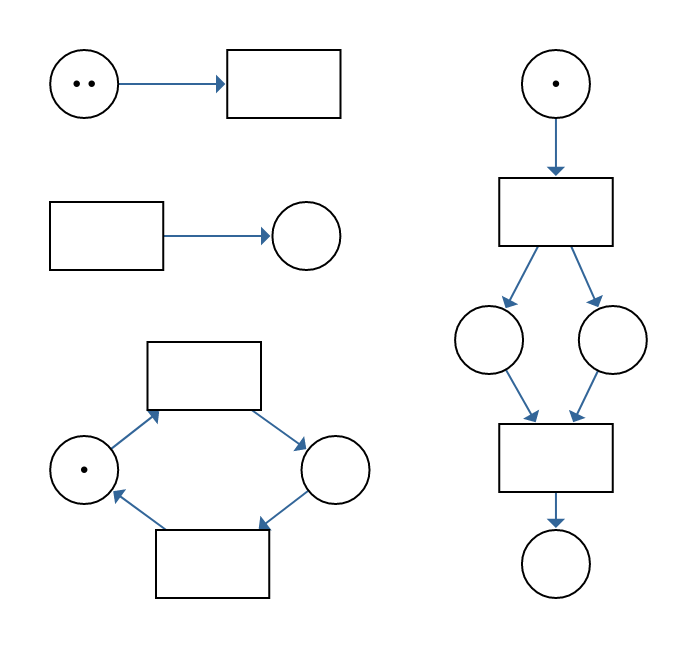
\includegraphics[width=.5\textwidth]{../diagrams/netExamples.png}
  \caption{Petri-Net examples}
  \label{net_examples}
\end{figure}
Figure \ref{net_examples} shows four example nets.
In the top left corner is a net with one place and one transition.
The place is marked with two tokens and is the only place in the transitions preset.
This means that the transition is enabled and can fire.
Since every firing consumes a token (no edge annotations mean an edge weight of one), the transition can fire exactly two times.
After that, the net will be dead.
The net below looks similar, only the edge direction is flipped.
Now the preset of the transition is empty.
The semantics here is that all places in the preset are properly marked resulting in a transition that can always fire.
As a result, the connected place can accumulate an unbounded amount of tokens.
The third net in the bottom left corner has a circular shape.
At any given time one of the two transitions can fire, virtually moving the token back and forth.
The token count in this net has an upper bound of one since both transitions always consume as many tokens as they produce and it initial marking has one token.
It also has no terminal state and can always fire one of the two transitions.
And the last net on the right shows that tokens indeed are produced and consumed, not moved.
The top transition will consume a token from the top place and produce two tokens, one on each place below.
After that the second transition will consume both tokens (one token from each place in the preset) and produce a token on the bottom most place.
It is not possible to consume only one of the two tokens -- every place from the preplace is involved in the firing of a transition!
And after the second transition has fired the net will be dead in a terminal state.

There is a large formal background to Petri-Nets that makes it possible to check for a variety of properties\cite{murata1989petri}.
For example, it can be analyzed if a particular marking can be reached from an initial marking or how many tokens a place may hold.
And -- important for this work -- if the net can reach a \textbf{dead} state, where no transition can fire anymore.
This state is equivalent to a deadlock.
Another nice feature of Petri-Net models is that, if a state is found where a property is satisfied, it is typically possible to find a witness path from the initial marking.


A downside of the formalism is the difficulty to model data.
This can be addressed with several additions that lead to \textbf{high level Petri-Nets}, where tokens are associated with additional properties that can represent data.
Transition in high level Petri-Nets can also respect the data of tokens in their firing behavior.
However, these additions to the formalism weaken the statements that can be derived from it, limiting the properties that can be checked for.

\subsection{Computational Tree Logic*}
\label{rel_ctl}
To articulate the properties we want to verify, we need a precise formalism for both state properties and properties of timing.
However, low-level Petri-Net have no time associated with transition firing;
Neither is there a defined duration between the firing of two transitions, nor a duration of a single firing.
So in our context the concept of time is not concerned with duration, but with the order of events.
Which transition fired before another; Or from which state another state can be reached.

These properties are commonly expressed in a \textbf{temporal logic}.
The primary ones used in model checking are linear temporal logic (LTL) from Pnueli\cite{pnueli1977temporal} computational tree logic (CTL) from Clarke and Emerson\cite{clarke1981design} and CTL* (the `*' is pronounced `star') from Emerson and Halpern\cite{emerson1985decision}(a super set which includes both LTL and CTL properties).
Since we will later use CTL* to formulate our properties, we will introduce its formula construction here.
A CTL* formula can be structured with the following elements:
\begin{itemize}
  \item The most basic CTL* formula is an \textbf{atomic proposition} (AP) which describes an atomic part of the system state, hence it is a \textbf{state formula} $\Phi$. 
  In our Petri-Nets this is typically a marking of a single place like $p_1$ is marked with 5 tokens: $p_1=5$, or $p_3$ has less than 3 tokens: $p_3<3$.
  \item Every state formula is also a \textbf{path formula} $\varphi$ which describe a sequence of events in a system.
  A plain state formula like from above describes the path to the initial state of the system. Such a formula is satisfied if the first state of the system satisfies the property (and makes no statement on the following states).
  \item Formulas can be combined to larger formulas with logic operators. For example: $!(p_1=5\ \&\ p_3<3)$.
  \item The \textbf{Next} operator $X\varphi$ describes a path to the successor state. For example: $p_1=5$ is satisfied if $p_5$ is marked with 5 tokens in the first state, $X(p_1=5)$ is satisfied if $p_5$ is marked with 5 tokens in the second state, $XX(p_1=5$) is satisfied if $p_5$ is marked with five tokens in the third state and so on.
  \item The \textbf{Eventually} operator $F\varphi$ describes a path formula that is satisfied if the enclosed formula is satisfied in some successor state or -- to formulate it differently: if it is reachable from the formula it is applied on.
  \item The \textbf{Always} operator $G\varphi$ describes a path formula that is satisfied if the enclosed formula is satisfied in every successor state -- or if it is always satisfied in the enclosed formula.
  \item The \textbf{Until} operator $\varphi_1 U\varphi_2$ describes a path formula that is satisfied if the formula $\varphi_1$ is satisfied in every state until a state is reached which satisfies $\varphi_2$ at least once.
  For example there is always an enabled transition in a circle (of the form $t_1\rightarrow p_1 \rightarrow ... \rightarrow t_n \rightarrow p_n \rightarrow t_1$) as long as at least one of the places is marked with a token.
  But it can be marked again later if all tokens where lost.
  % TODO: besipiele evtl mit bezug auf das petri net example
  \item And finally there are the \textbf{Path quantifiers} $E\varphi$ and $A\varphi$ which can be used to make a statement for the branching behavior of the system.
  Depending on a given state there might be multiple possible following states.
  In Petri-Nets that means there are multiple enabled transitions that can fire next.
  So depending on the actually firing transition, the resulting sequence of following states (the paths) can differ.
  If the \textbf{Universal path quantifier} $A\varphi$ is applied on a path formula the resulting formula is only satisfied if the path formula is satisfied in \textbf{all} branching paths.
  In contrast, the \textbf{Existential path quantifier} $E\varphi$ only requires the associated path formula to be satisfied in \textbf{one} of the successive paths.
\end{itemize}
The AP's and operators can be combined to express complex properties which serve as an input for model checkers.
